\section{Chemical and biological processes}\label{se:chemical_process}
This section will describe the chemical and biological processes that wastewater undergoes from the water is used to it is cleaned at the water treatment plant. The processes in a wastewater treatment plant will be investigated to get an understanding of the different processes. %Furthermore a illustration will be presented to elaborate the details in a sewer. 

Within wastewater there is an infinite number of living organisms before entering the WWTP. It contains from around 100.000 to 1.000.000 microorganisms per milliliter. Theses organisms originates from sanitary waste and soil. They are a natural living part of the organic matter and they are an important part of the cleansing, of the wastewater, at the WWTP. To be able to obtain a high water quality at the output of the WWTP it is necessary to have a thorough understanding of these microorganisms \cite{biological_wastewater}. % An acceptable cleansing of the wastewater is therefore depended on understanding the requirements for the most optimal conditions for the microorganisms. 

Nearly all of the microorganisms found in wastewater are not harmful and therefore does not cause a disease for mankind. However a small group of the microorganisms can cause diseases and these are of a great concern in wastewater treatment. The most known diseases are typhoid fever, dysentery, cholera, and hepatitis \cite{biological_wastewater}.

The microorganisms in the WWTP have a specific role in the decomposition of the waste. The three most notable microorganisms in the biological treatment process are bacteria, fungi and protozoa. The bacteria has the primary role of degrading the wastewater compounds, thereby producing sediment solids. Bacteria is a single cell organism and is capable of reproducing rapidly when in contact with water. They consume the waste by taking it through the cell wall \cite{biological_wastewater}. Fungi like bacteria decomposes the organic waste, however they also pose a significant problem for the wastewater treatment as the fungi can proliferate to an extent where it has detrimental consequences for the effluent quality \cite{fungi_source}. Lastly protozoa acts as predators toward the present bacterial population such that it can be controlled \cite{biological_wastewater}. 

% https://www.aquaenviro.co.uk/fungal-problems-in-wastewater-treatment-works/ kilde for fungus

In figure \ref{fig:sewer_overview_of_the_chemical_process} an illustration is shown of the processes that wastewater undergoes within the sewer.
\begin{figure}[H]
\centering
\includegraphics[width=1\textwidth]{report/introduction/pictures/detailed_sewer.pdf}
\caption{General overview of a sewer where the processes are illustrated. arbejdsblad billede. \fxnote{Ny tegning}}
\label{fig:sewer_overview_of_the_chemical_process}
\end{figure}

Wastewater are subject to a variety of mass changes in a sewer. One is due to free electrons in the wastewater, where different kinds of chemical reactions occurs. This results in different compounds being created which will be elaborated in subsection \ref{subse:chemical_reactions_in_a_sewer}. The concentration level and the chemical compounds, which exists at the inlet of the sewer, undergoes reactions in the sewer before reaching the WWTP. These reactions has the possibility to create gases which are released into the urban atmosphere, which is not ideal as it is typically malodorous. %Besides chemical reaction in the sewer there are also microorganisms. %The microorganisms consumes the sludge that sediments in the sewer and by consuming it they help break down the waste into inorganic and organic byproducts \cite{bacteria_sewer}. 
Microorganisms are reproducing on the biofilm that is created on the surface of the pipe. Furthermore the wastewater in the pipes can sink into the groundwater and the soils due to small leaks in the construction of the sewer \fxnote{Måske vi burde have noget med at grundvand faktisk også trænger ind i kloakkerne. Det kan være vigtigt i forbindelse med et statisk offset i vand flow når vi skal til at simulere.}. The wastewater ends up at the wastewater treatment plant, this process will be explained in subsection \ref{subse:Wastewater treatment plant}. And as previous mentioned in case of heavy precipitation to avoid flooding, the wastewater will be lead into receiving waters. 


\subsection{Chemical reactions in a sewer}\label{subse:chemical_reactions_in_a_sewer}
A wastewater treatment plant does not only receive what is discharged into the sewer from the industry and households but also the chemical and biological reactions that occurs in a sewer. The chemical reactions occur as redox reactions between the different compounds. Redox reaction is the transfer of electrons between two compounds at an atomic or molecular scale. By transferring electrons from one compound to another new compounds will arise, such as hydrogen sulfide which is know for its malodorous smell of rotten eggs. These reactions are determined by the electron acceptors that are present in the wastewater. The electron acceptor is the compound that receives electrons in a redox reaction. Examples of dissolved acceptors are oxygen ($O_2$), nitrate ($NO^-_3$) and sulfate ($SO^{2-}_4$), which is determined by whether aerobic, anoxic or anaerobic conditions occur in the sewer. The redox reaction reduces these three compounds in the wastewater by changing them to new compounds such as water ($H_2O$), molecular nitrogen ($N_2$) and hydrogen sulfide ($H_2S$) \cite{Sewer_processes}. 

Where redox reactions happens are, to a great extend, determined by the design of the sewer. The aerobic, anaerobic and anoxic conditions does not exist in the same part of the sewer, and the last only occurs if nitrate is artificially added to the wastewater. If the sewer is in an aerobic state then the typical characteristics for the sewer are either partly filled gravity sewer or an aerated pressure sewer. This means that there are free oxygen ($O^+$) molecules, and these will be connected with hydrogen to create water. If the sewer is in an anoxic state, which occurs in pressure sewers, then the addition of nitrate to the wastewater results in molecular nitrogen. If the sewer is in an anaerobic state the characteristic of the sewer is either a pressure sewer or a full flowing gravity sewer, then the reaction will result in hydrogen sulfide as the sulfate will bind with the hydrogen molecules. With the knowledge of these condition sewers can actively be designed to achieve a specific state \cite{Sewer_processes}. The two desired states in the sewers are aerobic in gravity sewers and anoxic in pressure sewers to avoid malodorous dissipation into the urban atmosphere.

\fxnote{Lav en table over disse 3 tilstande i kloakken}

%This knowledge is used to construct a simulation that is able to express the chemical and biological reaction which occur in wastewater. %A general model for describing the processes within a sewer is a extremely complex procedure, due to the variability in modeling, catchment characteristics and climate conditions which in practice are legion and therefore a general model formulation is not optimal. 
To model these chemical and biological reactions in sewers a model concept, Wastewater Aerobic/Anaerobic Transformation in Sewers (WATS), is used. The WATS model is expressed as differential mass balance equations that is suitable for numerical computation\fxnote{Hvad mener du med mere skarp her Thomas? i forhold til numerical computation} and can therefore be included in simulations for a specific objective e.g. model of water, biofilm and gas phase transformations. The WATS model can be applied to a variety of different sewers as long as a fundamental understanding of the sewer process is available. Whether it is aerobic, anoxic or anaerobic conditions that dominate the sewer, the soil composition and the pH concentration of the wastewater must also be included in the WATS model \cite{Sewer_processes}.     



%Furthermore turbulence in the flow of the wastewater affects reaeration and can release odorous and corrosive particles into the atmosphere \cite{Sewer_processes}.    

% \begin{figure}[H]
% \centering
% 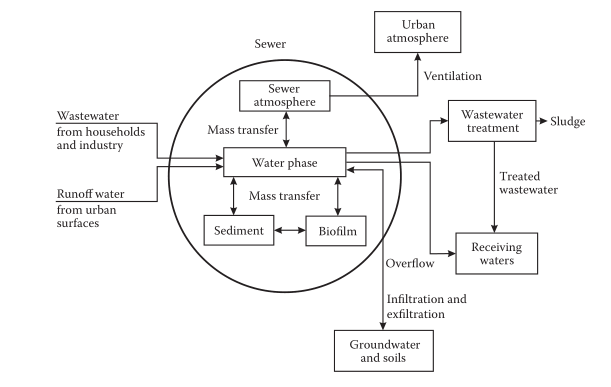
\includegraphics[width=1\textwidth]{report/introduction/pictures/sewer_overview_of_the_different_parts.png}
% \caption{Illustrates how the wastewater flows from the industry and households to the treatment plant. \fxnote{Ny tegning}}
% \label{fig:sewer_overview_of_the_different_parts}
% \end{figure}

\subsection{Wastewater treatment plant}\label{subse:Wastewater treatment plant}
Wasterwater from households and industry contains organic and inorganic matter and if it is release into the water environment it will result in a polluted environment. This can cause oxygen depletion and thereby affect the wildlife in the water environment negatively. Therefore the wastewater is lead to a WWTP to purify it from these substances which are harmful to the environment. In the following section the process that wasterwater undergoes in the WWTP will be elaborated. 

In figure \ref{fig:wwtp_process} the process wastewater undergoes is illustrated. 
\begin{figure}[H]
\centering
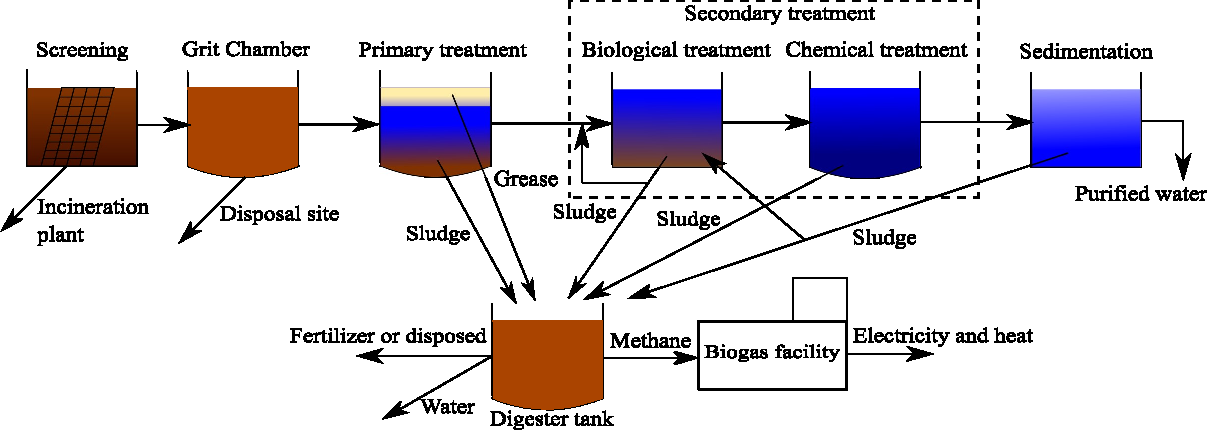
\includegraphics[clip, trim=0cm 13cm 9cm 0cm, width=1.00\textwidth]{report/introduction/pictures/WWTP_overview}
\caption{General overview of a wastewater treatment plant.}
\label{fig:wwtp_process}
\end{figure}

At the WWTP the wastewater undergoes several process before the organic and inorganic matters are removed. The first stage of purifying the wastewater is screening, where the larger objects are removed from the wastewater which would either block the flow or damage the equipment. Examples of objects that are filtered from the wastewater are bottles, plastic bags and diapers \cite{wwtp_process}. %These objects transported to a combustion facility.  %which basically is all items that would either block or damage the equipment. 

The wastewater is then lead into the primary treatment where it first will enter a grit chamber where objects as sand and stones will settle to the bottom of the tank. These grit chambers are crucial in WWTP that are connected with combined sewer systems.%, which means that the storm water from urbane surfaces is discharged into the same sewer as the human waste. 
The storm water may wash sand, stones, and gravel into the sewer and these objects will therefore be sorted out in this process \cite{epa_wwtp}. These objects are collected and disposed at a disposal site. 

After the screening and removal of grit the wastewater still contains organic and inorganic matter. By leading the wastewater into the primary treatment tank where the flow of the wastewater is reduced such that the organic matter will sediment in the tank, while the grease will accumulated at the top of the tank. The grease is then scrapped into the digester tank. The matter that have sedimented is now called sludge or raw primary biosolids. At the bottom of the tank large scrappers are moving the sludge to the center of the  tank where it is pumped into the digester tank \cite{epa_wwtp}. Water flows or is pumped into the secondary treatment. 

In the secondary treatment the water is lead into an aeration tank, this is called the biological treatment. By aeration of the wastewater the bacteria gain optimal conditions for respiration and thereby speed up the process of decomposing the remaining organic matter from the primary treatment process. In the process of decomposing the organic matter the bacterias will produce $CO_2$ that will dissipate into the atmosphere. Furthermore when the bacteria have consumed the organic matter they will start to produce heavier particles that will sediment in the tank \cite{wwtp_ekstra}. In figure \ref{fig:secondary_treatment} this process is illustrated.

%% https://www.youtube.com/watch?v=cEQ_INO6OlE


\begin{figure}[H]
\centering
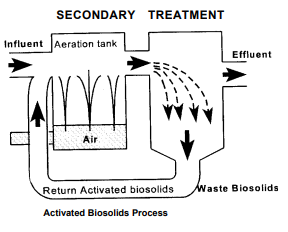
\includegraphics[width=.6\textwidth]{report/introduction/pictures/secondary_treatment.png}
\caption{Illustration of the secondary treatment process. arbejdsblad billede. \fxnote{Ny tegning}}
\label{fig:secondary_treatment}%https://www3.epa.gov/npdes/pubs/bastre.pdf
\end{figure} 

This is called the activated sludge process, because some of the sludge is reused in the aeration phase to keep a high bacteria population. This is done to have ad high s removal rate of pollutants in the wastewater as possible. The reused sludge contains millions of microorganisms that helps purifying the water. The sludge that have sedimented is pumped to the digester tank \cite{epa_wwtp}.

Hereafter a chemical treatment is performed to remove the inorganic matter that is left in the wastewater. This will create chemical reactions and thereby create new compounds that will sediment in the tank, which will be pumped into the digester tank. The chemical added to the process does not cause any damage to the environment \cite{youtube_wastewater}.

After these treatment processes there are still some particle left in the wastewater. It is lead through a sedimentation tank where the remaining bacteria and sludge will settle before released into receiving waters. The sedimented particles will either be pumped to the digester tank for further processes or reused in the activated sludge process.

% in tanks where a mixture of chemicals are used to purify the remaining water before leading it into the environment. The remaining particles will sediment creating more sludge. Hereafter the water is lead into the environment \cite{youtube_wastewater}. \fxnote{skal vi beskrive de her kemikalier? og hvilken process man start ved at tilføje nogle bestemte ting? Personligt vil jeg sige det er for meget. }

The sludge that is collected in the digester tank undergoes further treatment, where the remaining water in the sludge is separated from it. The water is lead back to the wastewater treatment process where it will undergo the same process again. The sludge is collected and used as fertilizer or disposed in a landfill and the gas created in the process can be used at a biogas facility to produce electricity and heat \cite{wwtp_ekstra}.


\section{Problem for the WWTP}
In the following section it will be shown how a daily input flow to the WWTP would like and what effects it can have on the purifying process. Furthermore the problems that comes with the industry will be explained. 

The WWTP in Fredericia purifies wastewater from the industry, households and urban surfaces. A general daily intake of wastewater is illustrated in figure \ref{fig:input_to_wwtp}  

\begin{figure}[H]
\centering
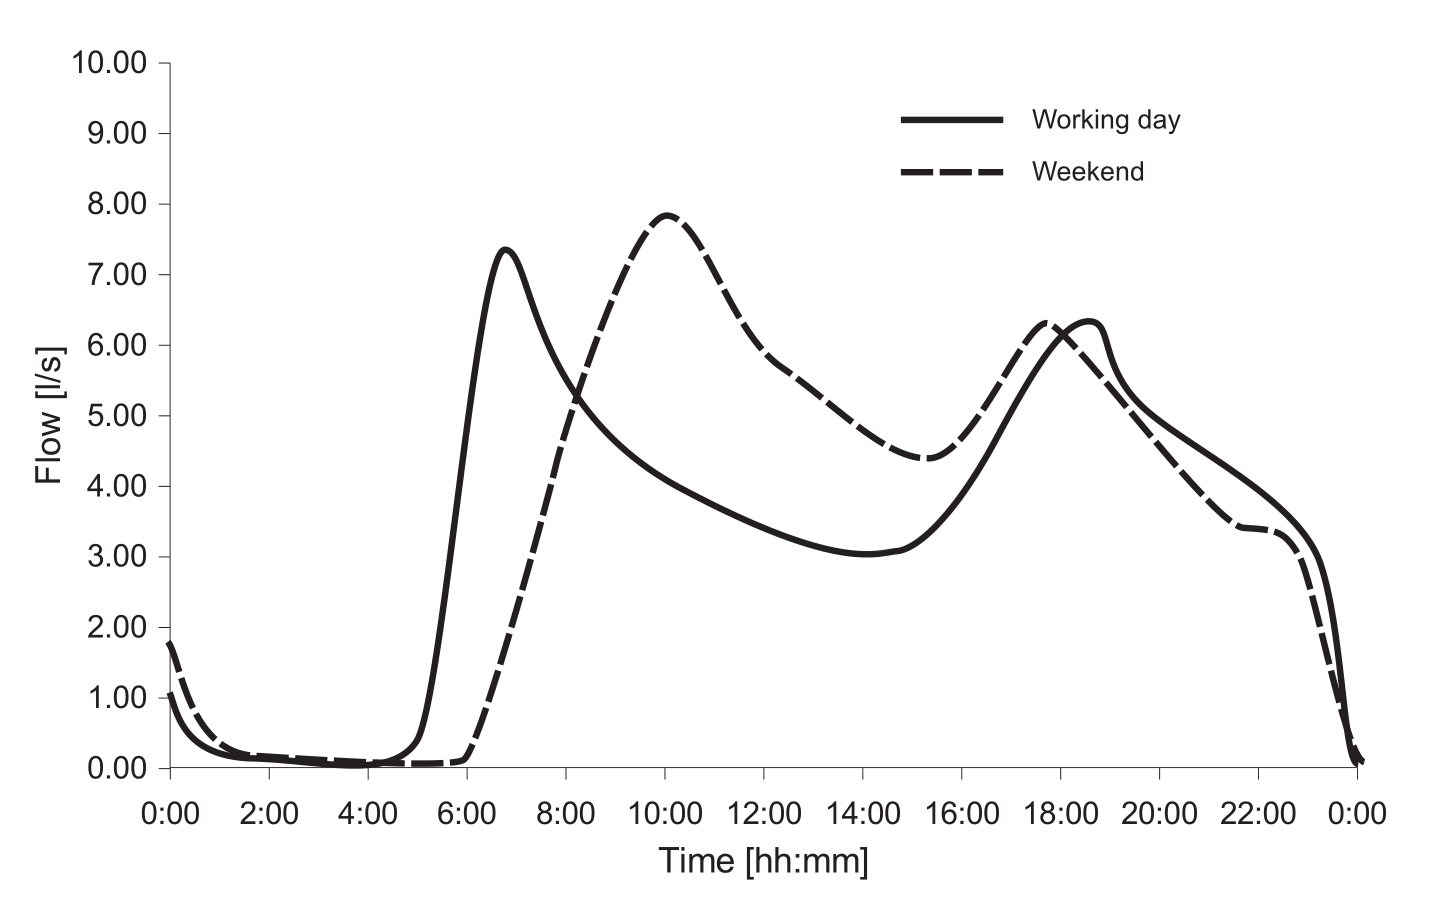
\includegraphics[width=.6\textwidth]{report/introduction/pictures/poopflow.png}
\caption{Typical daily flow pattern from the town Frejlev, with approximately 2000 habitants \cite{schlutter1999numerical}.}
%\caption{Input to the WWTP over a day, where the red line is showing the current input to the WWTP and the green is that wanted input. arbejdsblad billede. \fxnote{Ny tegning}}
\label{fig:input_to_wwtp}%https://www3.epa.gov/npdes/pubs/bastre.pdf
\end{figure} 

From around 06:00 there is a peak, it is due to people preparing for work, where the majority of wastewater comes from toilets visits and baths. Doing the day the flow slows down until people start to return from work where it has a flow increase due to cooking, baths, toilets etc. Doing night the flow is at a minimum as people are sleeping, however there is a constant intake of precipitation, throughout the pipeline, because it will sink through the ground and into sewer through the pipe wall.  

These spikes or increased flows at certain times results in a lower quality of the effluent that leaves the WWTP. The aeration phase where the process requires power to drive the pumps that create this oxygenation of the water. The process will have to follow the input flow to accommodate the changes. When the input is high the process requires a higher population of microorganisms to purify the wastewater, and therefore more air is needed in the wastewater. 

In Fredericia there are multiple big companies that empty their process out into the sewer. Must of the time the companies have a constant outlet to the sewer, however failure in the process at the company is know to occur. An example is the dairy where, in case of a bad batch, they are emptying their entire process of cream into the sewer. This a huge load for the WWTP to purify. It is known that the companies, in some cases, does not alert the WWTP about these load changes. 

This possess a huge problem WWTP as it does not have the capacity to purify the wastewater to achieve a acceptable output quality of the effluent. In the case where the load for the WWTP is to extreme and they are not able to process the wastewater through the normal process then to speed up the process to prevent overflow they only process the wastewater through a sedimentation phase and then let into the fjord. Furthermore the concentration of the matter that comes from the industry is also a problem for the WWTP, as it is in some cases very concentrated and therefore difficult to process.  

It is desired to have as constant as possible input into the WWTP to keep the aeration phase as constant as possible. Thereby reducing the energy cost in this phase and gain a more optimal purify process. Thereby obtaining a better water quality at the output of the plant. Furthermore the it is wanted to attenuate the concentration of the matter from the industry to a level where the WWTP purify it to obtain a sufficient water quality. 

%t is suggested from the department of ???? (Amelia) that buffer tanks should be placed though out the network. The idea is to hold back the wastewater and thereby control the output of these tanks to obtain a desired flow. 
% Skriv et argument for "en mere optimal rensnings process"      


%beskrive at vi gerne vil have et konstant indflow ind til WWTP, da selve iltningsprocessen så kan køres mere konstant, hvilket vil betyde energi besparelse. Kilde fra de to hoveder på Byggeri.
%Beskrive at industrierne bare smider deres affald ud uden at tænke over, hvad det har af indflydelse på resten af systemet. 

%Vis noget med flowet over en dag



